\section{Control system design}

\subsection{Problem a}

\todo{SPØR STUDASS HVORDAN man skal ta hensyn til $\psi$ i deloppgave b), c), og d). SVAR: Det er allerede tatt hensyn til ettersom psi holder seg innen 35 grader. Skriv om dette i svarene}

\todo{Can we get the figures closer to the text?}

The PD transfer function is of the form
\begin{align*}
    H_{pd}(s) &= K_{pd}(1+T_d s)/(1+T_f s) \\
              &= K_{pd}(1+T s)/(1+\alpha T s)
\end{align*}

Where $T_d = T$ in order to cancel the systems pole factor $(Ts + 1)$, and $T_f = \alpha T_d = \alpha T$. We set $K_{pd} = 0.8, \alpha = 0.1$. \Cref{fig:3a-bode_and_phasemargin} contains the bode plot of the system $H(s) = H_{ship}(s)H_{pd}(s)$, with the phase margin Pm at 48.3 degrees, and crossover angular frequency at 0.104 rad/s.

Phase margin was found through the $margin(sys)$ MATLAB function, by using trial and error in placing $K_{pd}$ and $\alpha$. The $margin$ function calculates the phase margin by solving for the difference between the system phase and -180 degrees at the angular frequency where the systems amplitude is 1. \todo{Skriv litt bedre om margin funksjonen}

\begin{figure}[ht]
    \centering
    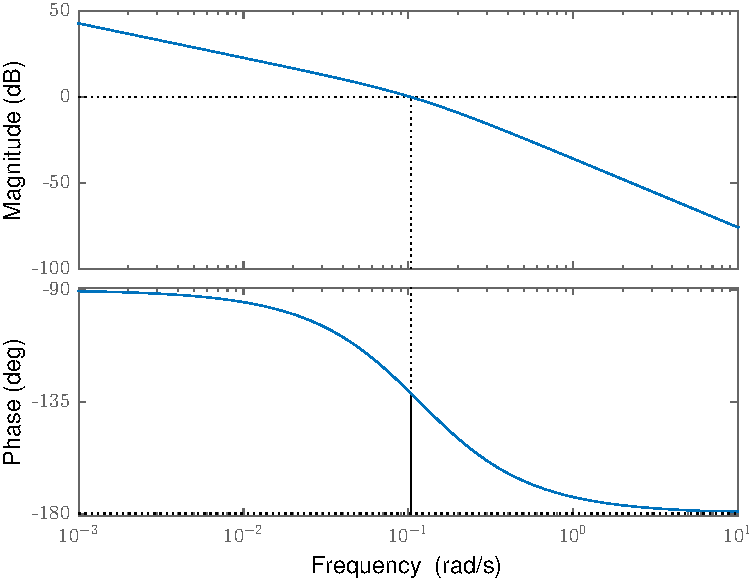
\includegraphics[width=0.5\textwidth]{images/3a-bode_and_phasemargin}
    \caption{Bode - and phase margin plot}
    \label{fig:3a-bode_and_phasemargin}
\end{figure}

\subsection{Problem b}
As shown in \cref{fig:3b-psi_and_rudder}, the autopilot functions well with only measurement noise.  It reaches the setpoint with acceptable inputs and minimal oscillations.

\begin{figure}[ht]
    \centering
    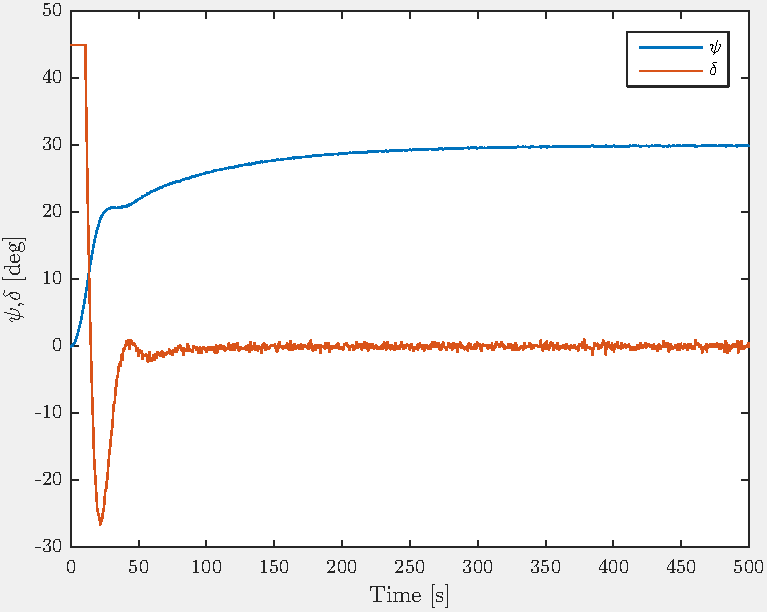
\includegraphics[width=0.5\textwidth]{images/3b-psi_and_rudder}
    \caption{Compass angle, $\psi$, and rudder angle, $\delta$, along the y-axis, plotted against time in the x-axis. With measurement noise}
    \label{fig:3b-psi_and_rudder}
\end{figure}

\subsection{Problem c}
With measurement noise and current disturbances, the autopilot functions as shown in \cref{fig:3b-psi_and_rudder_w_current}. While the angle approaches the setpoint with acceptable rudder inputs, there is an unacceptable steady state error, such that the angle never reaches the setpoint. This is expected since the current creates a bias in the rudder and there is no integral term in the controller to eliminate steady state errors.

\begin{figure}[ht]
    \centering
    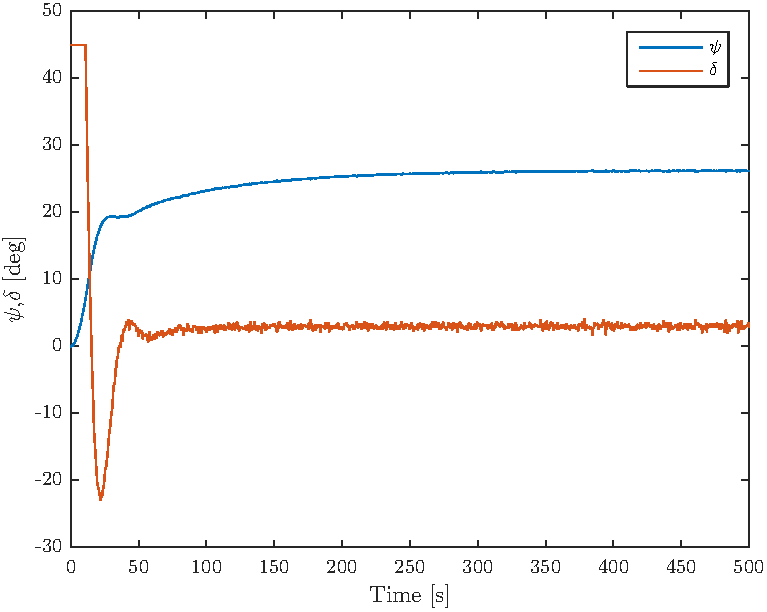
\includegraphics[width=0.5\textwidth]{images/3c-psi_and_rudder_w_current}
    \caption{Compass angle, $\psi$, and rudder angle, $\delta$, along the y-axis, plotted against time in the x-axis. With current disturbance and measurement noise}
    \label{fig:3b-psi_and_rudder_w_current}
\end{figure}

\subsection{Problem d}
With measurement noise, current and wave disturbances the autopilot functions as shown in \cref{fig:3b-psi_and_rudder_w_waves}. The controller reacts to the waves high frequency by creating unacceptable high frequency noise on the input. This would strain the motors and/or rudder of the ship. Furthermore, the heading does not settle on the setpoint, but rather oscillates around it in response to the waves. Since the disturbances are easily modeled, a filter could be used to reduce the noise in the controller. Therefore, the controller could better hold the ship's heading.

\begin{figure}[ht]
    \centering
    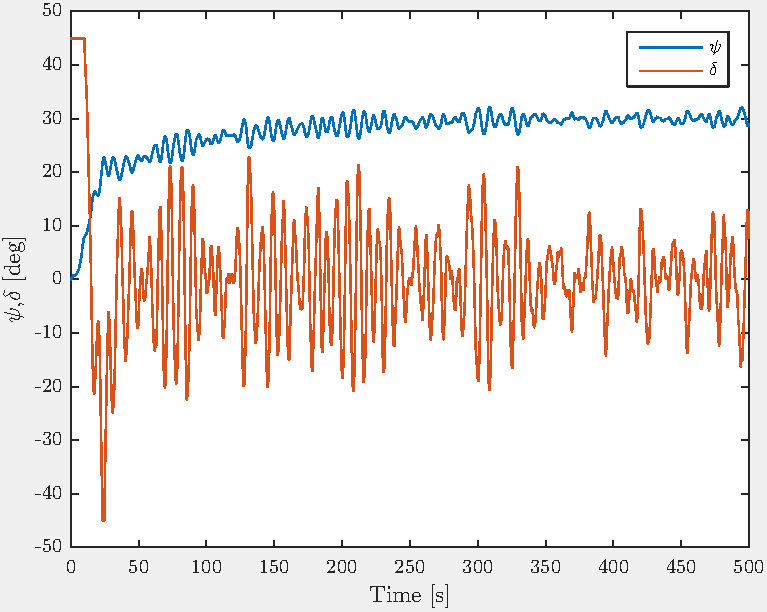
\includegraphics[width=0.5\textwidth]{images/3d-psi_and_rudder_w_waves}
    \caption{Compass angle, $\psi$, and rudder angle, $\delta$, along the y-axis, plotted against time in the x-axis. With wave disturbance and measurement noise}
    \label{fig:3b-psi_and_rudder_w_waves}
\end{figure}